\section{Rappels de POO}

\begin{frame}
    \begin{center}
    \fontsize{48pt}{7.2}\selectfont
    Rappels de POO
    \end{center}
\end{frame}

\subsection{Objet}
\begin{frame}
\frametitle{Qu'est-ce qu'un objet ?}
Un \underline{objet} est une structure de \textbf{donn\'{e}es} qui r\'{e}pond \`{a} un ensemble de \textbf{messages}.
\\~\\
Les \underline{donn\'{e}es} sont appel\'{e}es \textbf{champs} (fields).
\\
Les \underline{messages} compris par un objet sont repr\'{e}sent\'{e}s par des fonctions de cet objet appel\'{e}es \textbf{m\'{e}thodes}.
\end{frame}

\begin{frame}[fragile]
\frametitle{Interface}
\begin{lstlisting}
public interface House {

	void addResident(Human resident);

	void removeResident(String name);

	int countResidents();
}
	\end{lstlisting}
\end{frame}

\begin{frame}[fragile]
\frametitle{Classe}
\begin{lstlisting}
import java.util.ArrayList;
import java.util.List;

public class CityHouse implements House {
	private final List<Human> residents = new ArrayList<>();

	public void addResident(Human resident) {
		if(!residents.contains(resident) {
			residents.add(resident);
		}
	}
	public void removeResident(String name) {
		residents.removeIf(h -> h.getName().equals(name));
	}
	public int countResidents() {
    	return residents.size();
    }
}
	\end{lstlisting}
\end{frame}

\begin{frame}[fragile]
\frametitle{Instance}
\begin{lstlisting}
public class HouseApplication {
	public static void main(String[] args) {
		House _21_jump_street = new CityHouse();

		_21_jump_street.addResident(new Human("Channing Tatum"));
		_21_jump_street.addResident(new Human("Jonah Hill"));

		System.out.println("Number of residents: " + _21_jump_street.countResidents()); // 2

		_21_jump_street.addResident(new Human("Jonah Hill"));

		System.out.println("Number of residents: " + _21_jump_street.countResidents()); // 2
	}
}
	\end{lstlisting}
\end{frame}

\subsection{S O L I D}

\begin{frame}
	\frametitle{S O L I D}
	\begin{itemize}
    	\item \textbf{S}ingle responsibility: une seule responsabilit\'{e} par classe
		\item \textbf{O}pen/Close: ouvert \`{a} la composition, ferm\'{e} \`{a} la modification
		\item \textbf{Liskov} substitution: substitution par un sous-type sans modification de la coh\'{e}rence
		\item \textbf{I}nterface segregation: une interface (contrat) diff\'{e}rente par client
		\item \textbf{D}ependency inversion: travailler avec la forme la plus abstraite d\'{}un objet (une interface en g\'{e}n\'{e}ral)
    \end{itemize}
    ~\\
    La programmation orient\'{e}e objet n'est r\'{e}ellement int\'{e}ressante qu'en mettant en \oe{}uvre les principes \textbf{S O L I D}.
\end{frame}

\begin{frame}[fragile]
	\frametitle{S O L I D: exemple I (L \& S)}
	\begin{lstlisting}
public interface Logger {
	void log(Level level, String message);
}
	\end{lstlisting}
    \begin{lstlisting}
public class ConsoleLogger implements Logger {
	public void log(Level level, String message) {
		System.out.prinln("[" + level + "] " + message);
	}
}
	\end{lstlisting}
    \begin{lstlisting}[basicstyle=\tiny]
public class FileLogger implements Logger {
	...
    public void log(Level level, String message) {
        try {
            Files.write(path, ("[" + level + "] " + message + "\n").getBytes(), APPEND, CREATE);
        } catch (IOException e) {
            throw new RuntimeException("Cannot write log message to file [" + path + "]", e);
        }
    }
}
	\end{lstlisting}
\end{frame}

\begin{frame}[fragile]
	\frametitle{S O L I D: exemple II (O \& D)}
	\begin{lstlisting}
import java.util.Arrays;

public class CompositeLogger implements Logger {

	private Iterable<Logger> delegates;

	public CompositeLogger(Logger... loggers) {
		this.delegates = Arrays.asList(loggers);
	}

	public void log(Level level, String message) {
		delegates.forEach(l -> l.log(level, message));
	}
}
	\end{lstlisting}
\end{frame}

\begin{frame}[fragile]
	\frametitle{S O L I D: exemple III (usage)}
	\begin{lstlisting}[basicstyle=\tiny]
import java.io.IOException;
import java.net.InetSocketAddress;
import java.net.Socket;

public class MyApplication {

	private static final Logger LOGGER = LoggerFactory.getLogger();

	public static void main(String[] args) {
		LOGGER.log(Level.INFO, "Application starts");

		String hostname = "google.com";
		int port = 80;
		int connectionTimeout = 2000; // in ms

		try (Socket socket = new Socket()) {
			socket.connect(new InetSocketAddress(hostname, port), connectionTimeout);
			LOGGER.log(Level.INFO, "Successfully connected to " + hostname);
		} catch (IOException e) {
			LOGGER.log(Level.ERROR, "Unable to connect to " + hostname + ": " + e.getMessage());
		}

		LOGGER.log(Level.INFO, "Application stops");
	}
}
	\end{lstlisting}
\end{frame}

\subsection{Thread}

\begin{frame}
	\frametitle{Qu'est-ce qu'un thread ?}
	Un \textbf{thread} est un fil d'ex\'{e}cution repr\'{e}sentant une t\^{a}che \`{a} effectuer.
    \\~\\
    La notion de thread est n\'{e}cessaire pour mod\'{e}liser des t\^{a}ches \`{a} r\'{e}aliser en parall\`{e}le.
    \begin{itemize}
    	\item un thread n\'{}est pas li\'{e} \`{a} un processeur
		\item il peut donc y en avoir plus que de processeurs (c\oe{}urs)
        \item un thread a \textit{globalement} deux \'{e}tats:
        \begin{itemize}
        	\item consommant du CPU
            \item attendant une notification
        \end{itemize}
        \item ex\'{e}cuter plusieurs threads sur un m\^{e}me processeur (c\oe{}ur) est co\^{u}teux
    \end{itemize}
    ~\\
    
\includegraphics[width=1cm]{img/karadoc.png}
    \begin{quote}
    \`{A} utiliser en toute technique d'arrosage donc
    \end{quote}
\end{frame}

\begin{frame}[fragile]
	\frametitle{Thread: Patron Object Pool}
    Il est possible d'utiliser la classe {\lstinline[basicstyle=\ttfamily\color{blue}]|java.lang.Thread|} afin de lancer directement un thread.
    \\~\\
    % Malformul\'{e}
    Cependant la fa\c{c}on la plus commune de g\'{e}rer ses threads depuis \textbf{Java 5} est d'utiliser le patron de conception \textbf{Object Pool} disponible via l'interface {\lstinline[basicstyle=\ttfamily\color{blue}]|java.util.concurrent.ExecutorService|}.
    \\~
    \begin{lstlisting}[basicstyle=\tiny]
import java.util.concurrent.*;

...
	public static void main(String[] args) throws InterruptedException {
		Runnable task1 = () -> System.out.println("Hello");
		Runnable task2 = () -> System.out.println("World");

		ExecutorService pool = Executors.newFixedThreadPool(2);

		try {
			pool.submit(task1);
			pool.submit(task2);
			pool.awaitTermination(100L, TimeUnit.MILLISECONDS);
		} finally {
			pool.shutdown();
		}
	}
	\end{lstlisting}
\end{frame}

\begin{frame}[fragile]
	\frametitle{Thread Safety}
    \begin{lstlisting}
private int counter = 0;

public int increment() {
    int tmp = counter;
    tmp = tmp + 1;
    counter = tmp;
    return tmp;
}
	\end{lstlisting}
    Solutions:
    \begin{itemize}
    	\item verrous ({\lstinline[basicstyle=\ttfamily\color{blue}]|synchronized|})
        \item types atomiques ({\lstinline[basicstyle=\ttfamily\color{blue}\small]|AtomicBoolean|}, etc.)
    \end{itemize}
    
    Il existe \'{e}galement le mot-cl\'{e} {\lstinline[basicstyle=\ttfamily\color{blue}]|volatile|} permettant d'obtenir la valeur "\`{a} jour" d\'{}une variable et non la valeur dans le cache du processeur.
    \\~\\
    {\lstinline[basicstyle=\color{red}]|Attention|} cependant, {\lstinline[basicstyle=\ttfamily\color{blue}]|volatile|} ne garantie pas l\'{}atomicit\'{e} des op\'{e}rations effectu\'{e}es sur la variable.
\end{frame}

\begin{frame}[fragile]
	\frametitle{Outillage pour manipuler des threads}    
    Il existe plein de bonnes choses dans le \textit{package} {\lstinline[basicstyle=\ttfamily\color{blue}]|java.util.concurrent|} permettant de contr\^{o}ler des threads
    \begin{itemize}
    	\item {\lstinline[basicstyle=\ttfamily\color{blue}]|Executors|}
    	\item {\lstinline[basicstyle=\ttfamily\color{blue}]|Semaphore|}
    	\item {\lstinline[basicstyle=\ttfamily\color{blue}]|CyclicBarrier|}
        \item {\lstinline[basicstyle=\ttfamily\color{blue}]|CompletableFuture|}
        \item ...
    \end{itemize}
    ~\\
    Il existe aussi des librairies d\'{e}di\'{e}es au \textit{flow control}
    \begin{itemize}
    	\item RxJava
    	\item Spring\'{}s{\lstinline[basicstyle=\ttfamily\color{blue}]| @Async|}
        \item librairies autours de NIO2 ({\lstinline[basicstyle=\ttfamily\color{blue}]|java.nio.*|})
        \item ...
    \end{itemize}
\end{frame}

\subsection{Collections}
\begin{frame}[fragile]
	\frametitle{Collections}
    Une collection est un ensemble d\'{}objet de m\^{e}me type.
    \\~\\
    % Ce sont presque des objets. Ils ne peuvent pas \^{e}tre \'{e}tendus, n'ont pas de nom de classe, sont utilis\'{e}s avec une syntaxe qui leur est propre, et ils h\'{e}ritent des m\'{e}thodes de la classe Object, notamment toString()
    Contrairement \`{a} un tableau, la taille d'une collection peut changer par l'ajout ou la suppression d\'{}\'{e}l\'{e}ments.
    \\~\\
    Une {\lstinline[basicstyle=\ttfamily\color{blue}]|Collection|} est {\lstinline[basicstyle=\ttfamily\color{blue}]|Iterable|}.
    \\~\\
    Cela signifie qu'elle doit renvoyer un objet {\lstinline[basicstyle=\ttfamily\color{blue}]|Iterator|}.
    \\~\\
    Un {\lstinline[basicstyle=\ttfamily\color{blue}]|Iterator|} va permettre d\'{}it\'{e}rer sur les \'{e}l\'{e}ments contenus dans la collection.
\end{frame}

\begin{frame}[fragile]
	\frametitle{Relations entre les classes de Collection}
    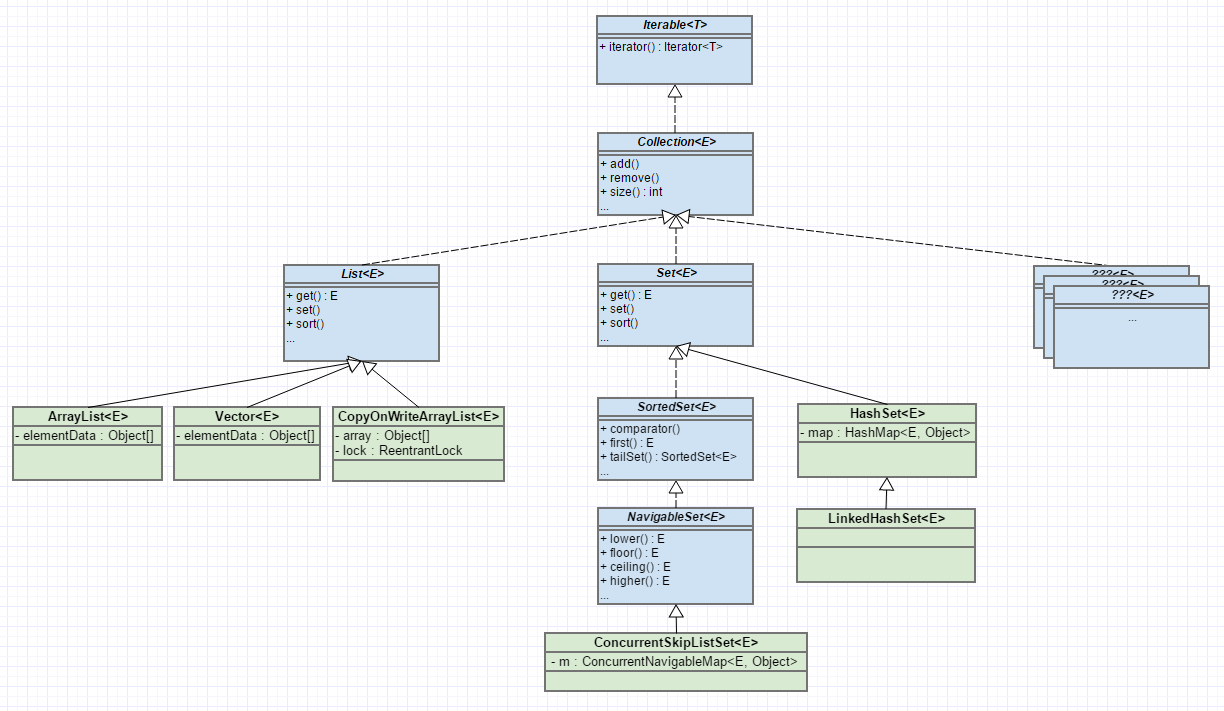
\includegraphics[width=11cm]{img/collections.png}
\end{frame}

\begin{frame}[fragile]
	\frametitle{Collections en Java}
    \begin{itemize}
      \item Une collection est un type \textit{g\'{e}n\'{e}rique}
      \item Le type d\'{}objet contenu est indiqu\'{e} entre chevron
      \item L\'{}interface de plus haut niveau est utilis\'{e}e pour les types des variables et des param\`{e}tres
    \end{itemize}
    ~\\
    \begin{lstlisting}
private final List<Human> humans = new ArrayList<Human>();

public boolean isAnyNameContained(Set<String> names) {
	return humans.stream()
		.filter(h -> names.contains(h.name))
		.findAny()
		.isPresent();
}
	\end{lstlisting}
    Ici le param\`{e}tre {\lstinline[basicstyle=\ttfamily\color{blue}]|Set<String> names|} impose \`{a} l'utilisateur un argument sans doublon.
\end{frame}
